% = = = = = = = = = = = = = = = = = = = = = %
%             Design Description            %
% = = = = = = = = = = = = = = = = = = = = = %

\let\clearpage\relax
\chapter{Final Design Description \& Analysis}

In this chapter, we will review our selected concepts in details, including engineering design analysis, design description and analysis of microarchitecture for each pipeline stages.

\section{Engineering Design Analysis}

\subsection{ISA} %sj
As we mentioned above, we will select our instruction set architecture (ISA) among three choices: MIPS, ARMv7 and RISC-V. Their advantages and disadvantages are listed in Section \ref{section:isa}.

After discussion, we decide to choose RISC-V ISA as our design standard.

Since our final product uses approximate computing unit to accelerate machine learning and neural network, custom ISA is necessary for us. RISC-V supports custom design instructions and also has enough design space compared to other two choices.

Besides, we need to balance our workload and supported features. RISC-V supports many pre-defined instructions, with acceptable complexity. After evaluation, we think we can finish our design and implement on RISC-V in three months.

\subsection{Microarchitecture} \label{section:Microarchitecture}% sl 
We have used the decision matrix to determine the final design of our processor microarchitecture design. Specifically, we determine to implement superscalar and out-of-order features in our design, which matches most of customer requirements. For example, in the aspect of performance, our superscalar out-of-order design provides good performance especially in those computing-intensive tasks. It matches the engineering specifications we set earlier, including supporting instruction dynamic scheduling, etc., and provides a good performance-power-cost balance.

\section{Design Description of ISA} % lzy - consider moving customized instructions to here

\section{Design Description of Microarchitecture}
In this part, we will explain our design details of each microarchitecture pipeline stages. A simplified pipeline design diagram is shown in Fig.~\ref{fig:pipeline}. Our processor supports 4-way superscalar execution and instruction dynamic scheduling, dividing into two parts: frontend and backend. In the frontend, there are 4 stages: instruction fetch (IF), instruction decode (ID), register renaming (RR), dispatch (DP). In the backend, there are 5 stages: issue (IS), register file (RF), execution (EX), write back (WB), and commit (CM).

\begin{figure}
    \centering
    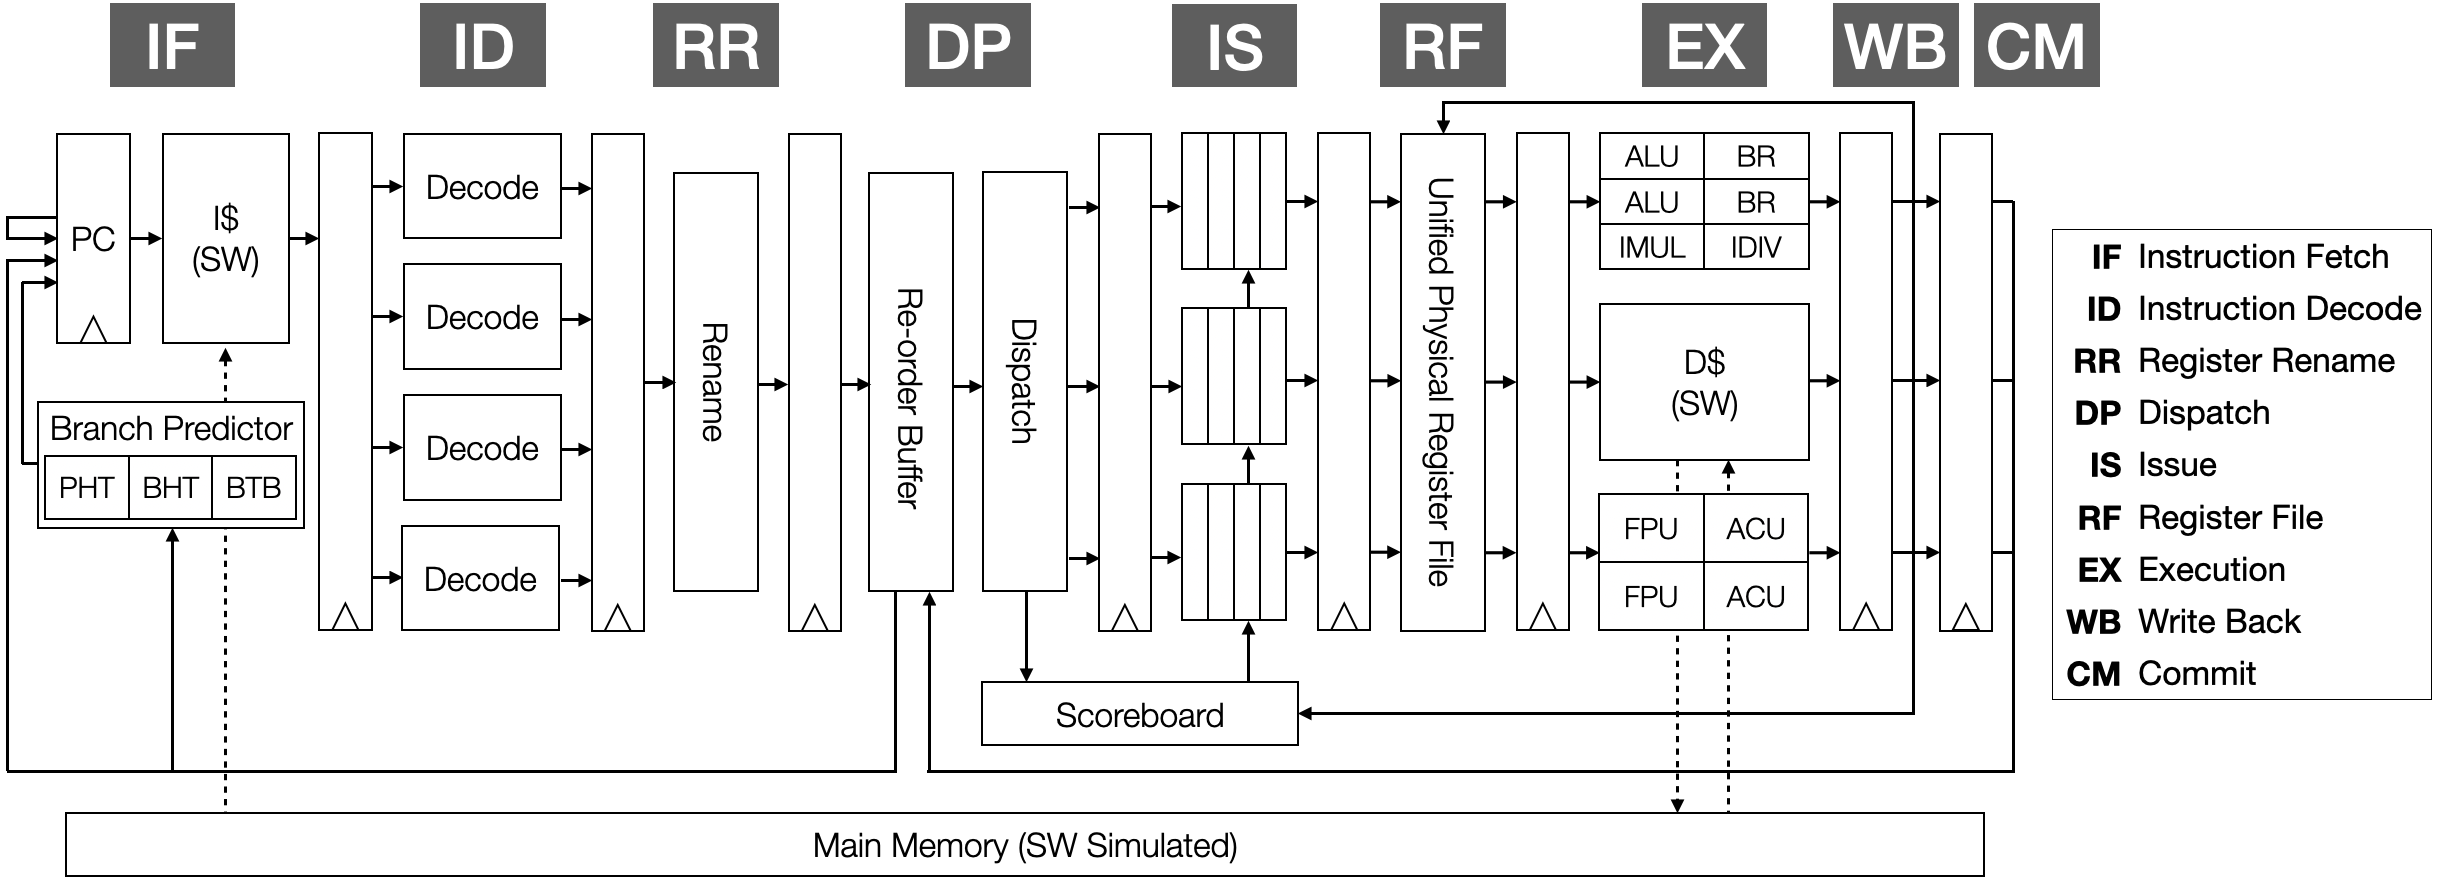
\includegraphics[width=\textwidth]{figure/design.png}
    \caption{Simplified pipeline diagram.}
    \label{fig:pipeline}
\end{figure}

\subsection{Instruction Fetch \& Branch Prediction} % syq
The Instruction Fetch stage is the first stage of the whole pipeline (Fig. \ref{fig:pipeline}). It reads instructions from memory. The branch predictor is also included into this stage. As is shown in Fig. \ref{fig:br_pred}, the branch predictor consists of Direction Predictor and Branch Target Table (BTB). The Direction Predictor uses 2 bits to represent the possibility of branch taken: 00 - strongly not taken, 01 - weakly not taken, 10- weakly taken, 11- strongly taken. We decides what is the next PC to read based on the mis-predict feedback from Reorder Buffer and the predict output of the branch predictor.
\begin{figure}[!htp]
    \centering
    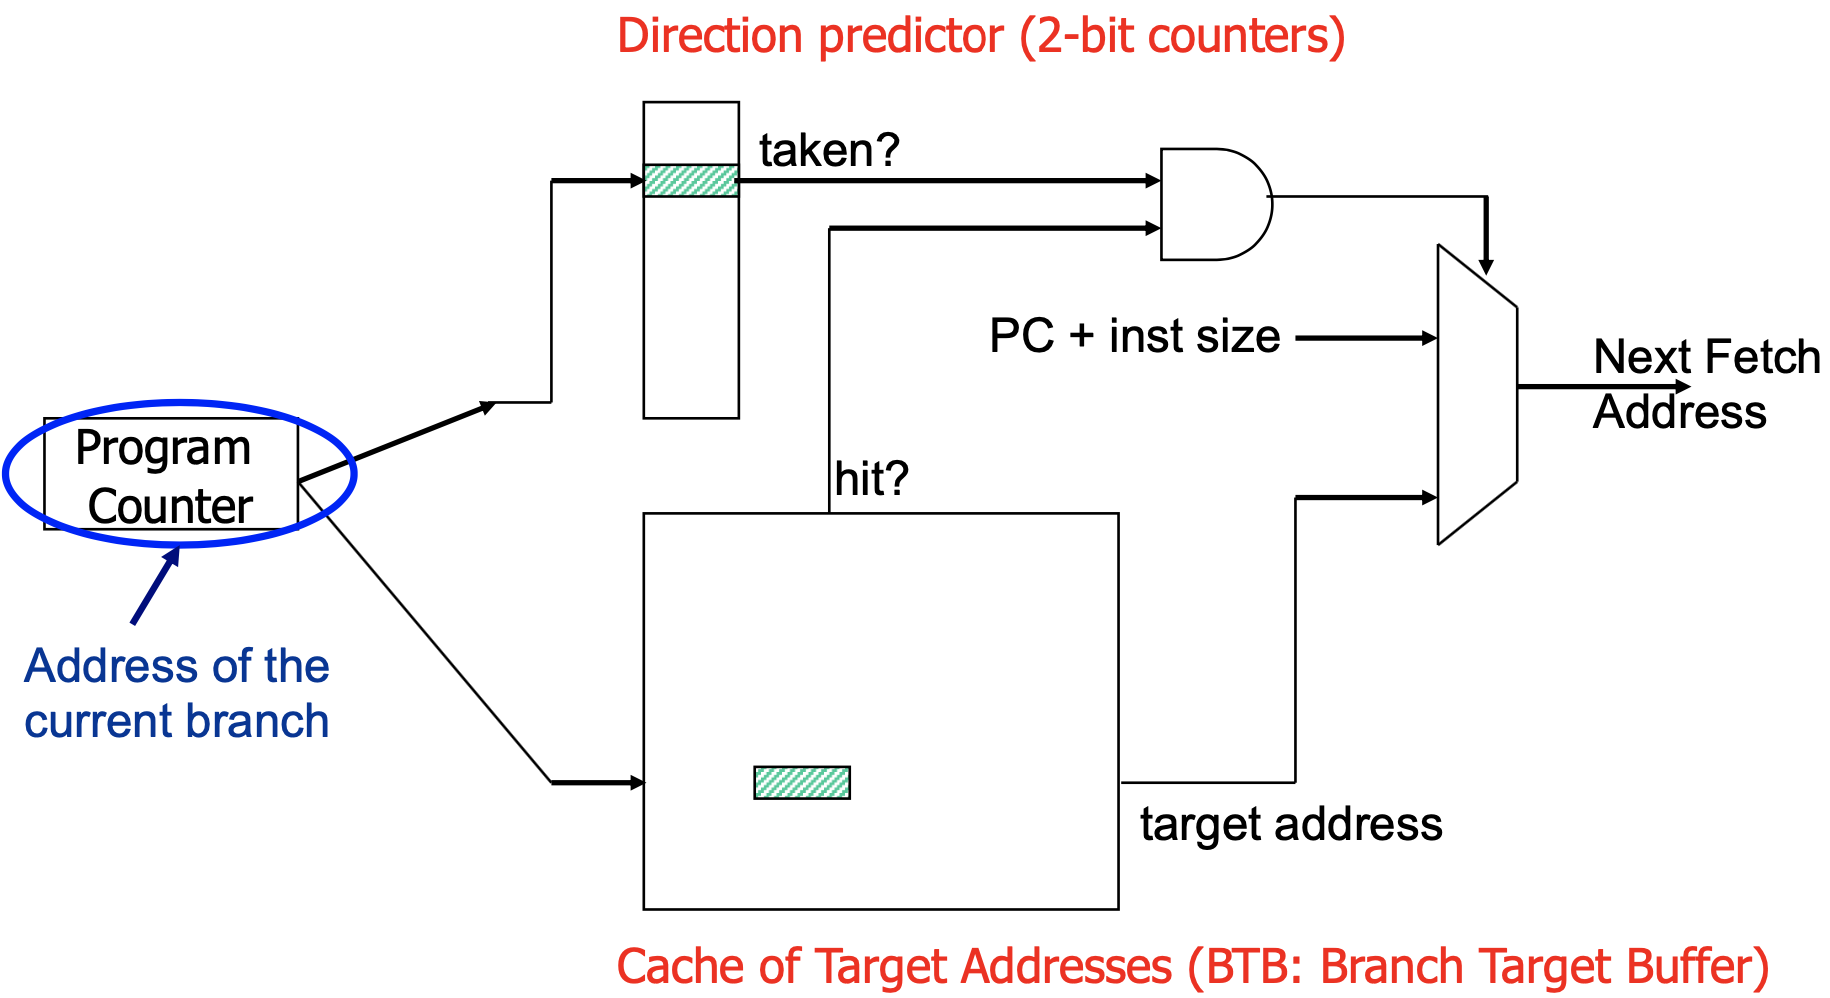
\includegraphics[width=0.8\textwidth]{figure/branch_predictor.png}
    \caption{Branch predictor diagram.}
    \label{fig:br_pred}
\end{figure}

\subsection{Fetch Buffer} % syq
The Fetch Buffer serves as a buffer to store the fetched instructions if they can not be dispatched at once due to the congestion of later stages. The buffer is implemented as a First-In-First-Out (FIFO) queue to ensure an in-order dispatch of instructions.

\subsection{Instruction Decode} %sj
In this part, we decode the input instructions into micro operations (\texttt{uops}). We use four decoders to make sure that four instructions can be decoded at the same time.

\begin{figure}[!htp]
    \centering
    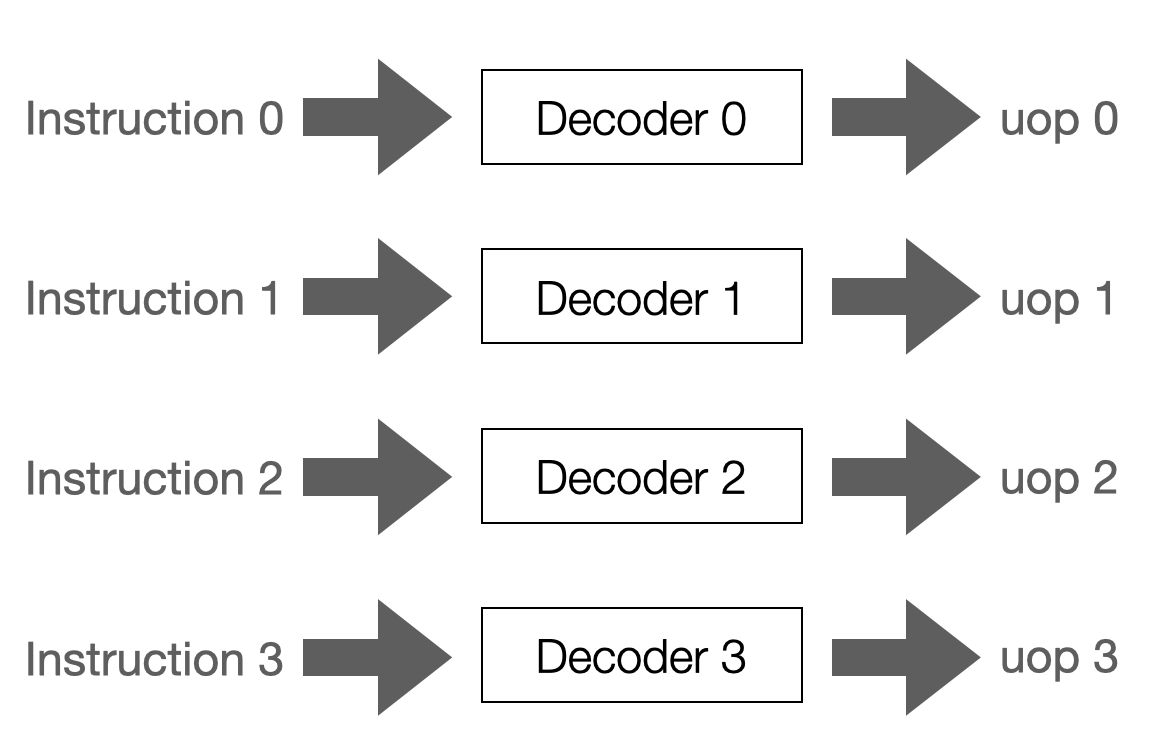
\includegraphics[width=0.5\textwidth]{figure/decode.png}
    \caption{4-way decoder.}
    \label{fig:decoder}
\end{figure}

RISC-V instructions can be classified by their formats. Fig.~\ref{fig:RISCV_inst} shows all instruction types. The decoders will first sort input instructions according to the format table. Then, the decoders will analyze information in each part of the instruction and translate them into micro operations that can be understood by the following stages.

\begin{figure}[!htp]
    \centering
    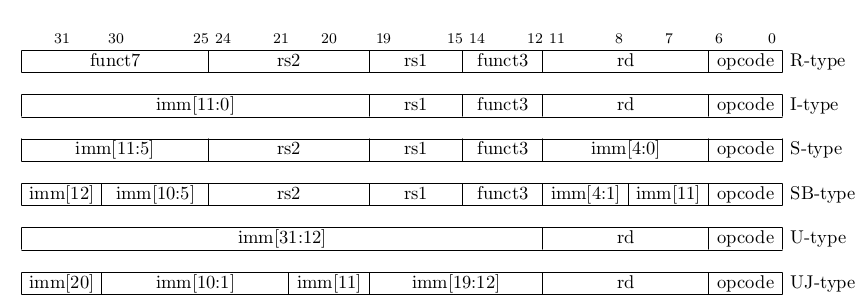
\includegraphics[width=0.85\textwidth]{figure/riscv-isa.png}
    \caption{RISC-V instruction format\cite{RISC-V_unprivileged_ISA}.}
    \label{fig:RISCV_inst1}
\end{figure}

Micro operations are designed as a data structure, including source architectural registers, destination register, used immediate and operation code. Therefore, other stages can fetch needed information quickly and accurately from micro operations.

\subsection{Register Rename} % sj
In this part, we rename architectural registers and assign them with physical registers. Besides, the rename part should also free physical registers that are retired by committed instructions.

The main purpose of register rename is to break the anti-dependency (write after read, WAR) and output dependency (write after write, WAW) between architectural registers. Therefore, instructions with these dependencies can be pipe-lined together in execution stage, which will improve the performance of the processor. Fig.~\ref{fig:waw_war} shows how to break WAR and WAW in the rename stage. On the other hand, the rename part should protect and record the true dependency (read after write, RAW) so that an instruction can read and get the right source register. For special architectural register, i.e., \texttt{x0}, the rename part should protect it to be assigned to other physical registers.

\begin{figure}[!htp]
    \centering
    
\includegraphics[width=0.5\textwidth]{figure/waw.png}
    
\includegraphics[width=0.5\textwidth]{figure/war.png}
    \caption{Write after read and write after write dependency.}
    \label{fig:waw_war}
\end{figure}

Our rename part is an ``explicit renaming'' or ``physical register file'' out-of-order core design. A physical register file (128 entries), containing many more registers than the ISA dictates (32 entries for integer and 32 entries for floating points), holds both the committed architectural register state and speculative register state. The retirement rename allocation table (rRAT) contains the information needed to recover the committed state. The mapping relation will be recorded in the mapping table, also called rename allocation table (RAT). As instructions are renamed, their register specifiers are explicitly updated to point to physical registers located in the physical register file. Fig.~\ref{fig:rename} shows the rename logic between two instructions and their architectural registers. Since our rename stage has four ways and can rename four instructions at the same time, the final logic is far more complex than the given example.

Since we use unified physical register file in issue stage, integer architectural registers and floating point architectural registers share the same register ``pool'' and address structure. For this reason, we also rename their physical registers together and do not take their differences into consideration in rename stage.

\begin{figure}[!htp]
    \centering
    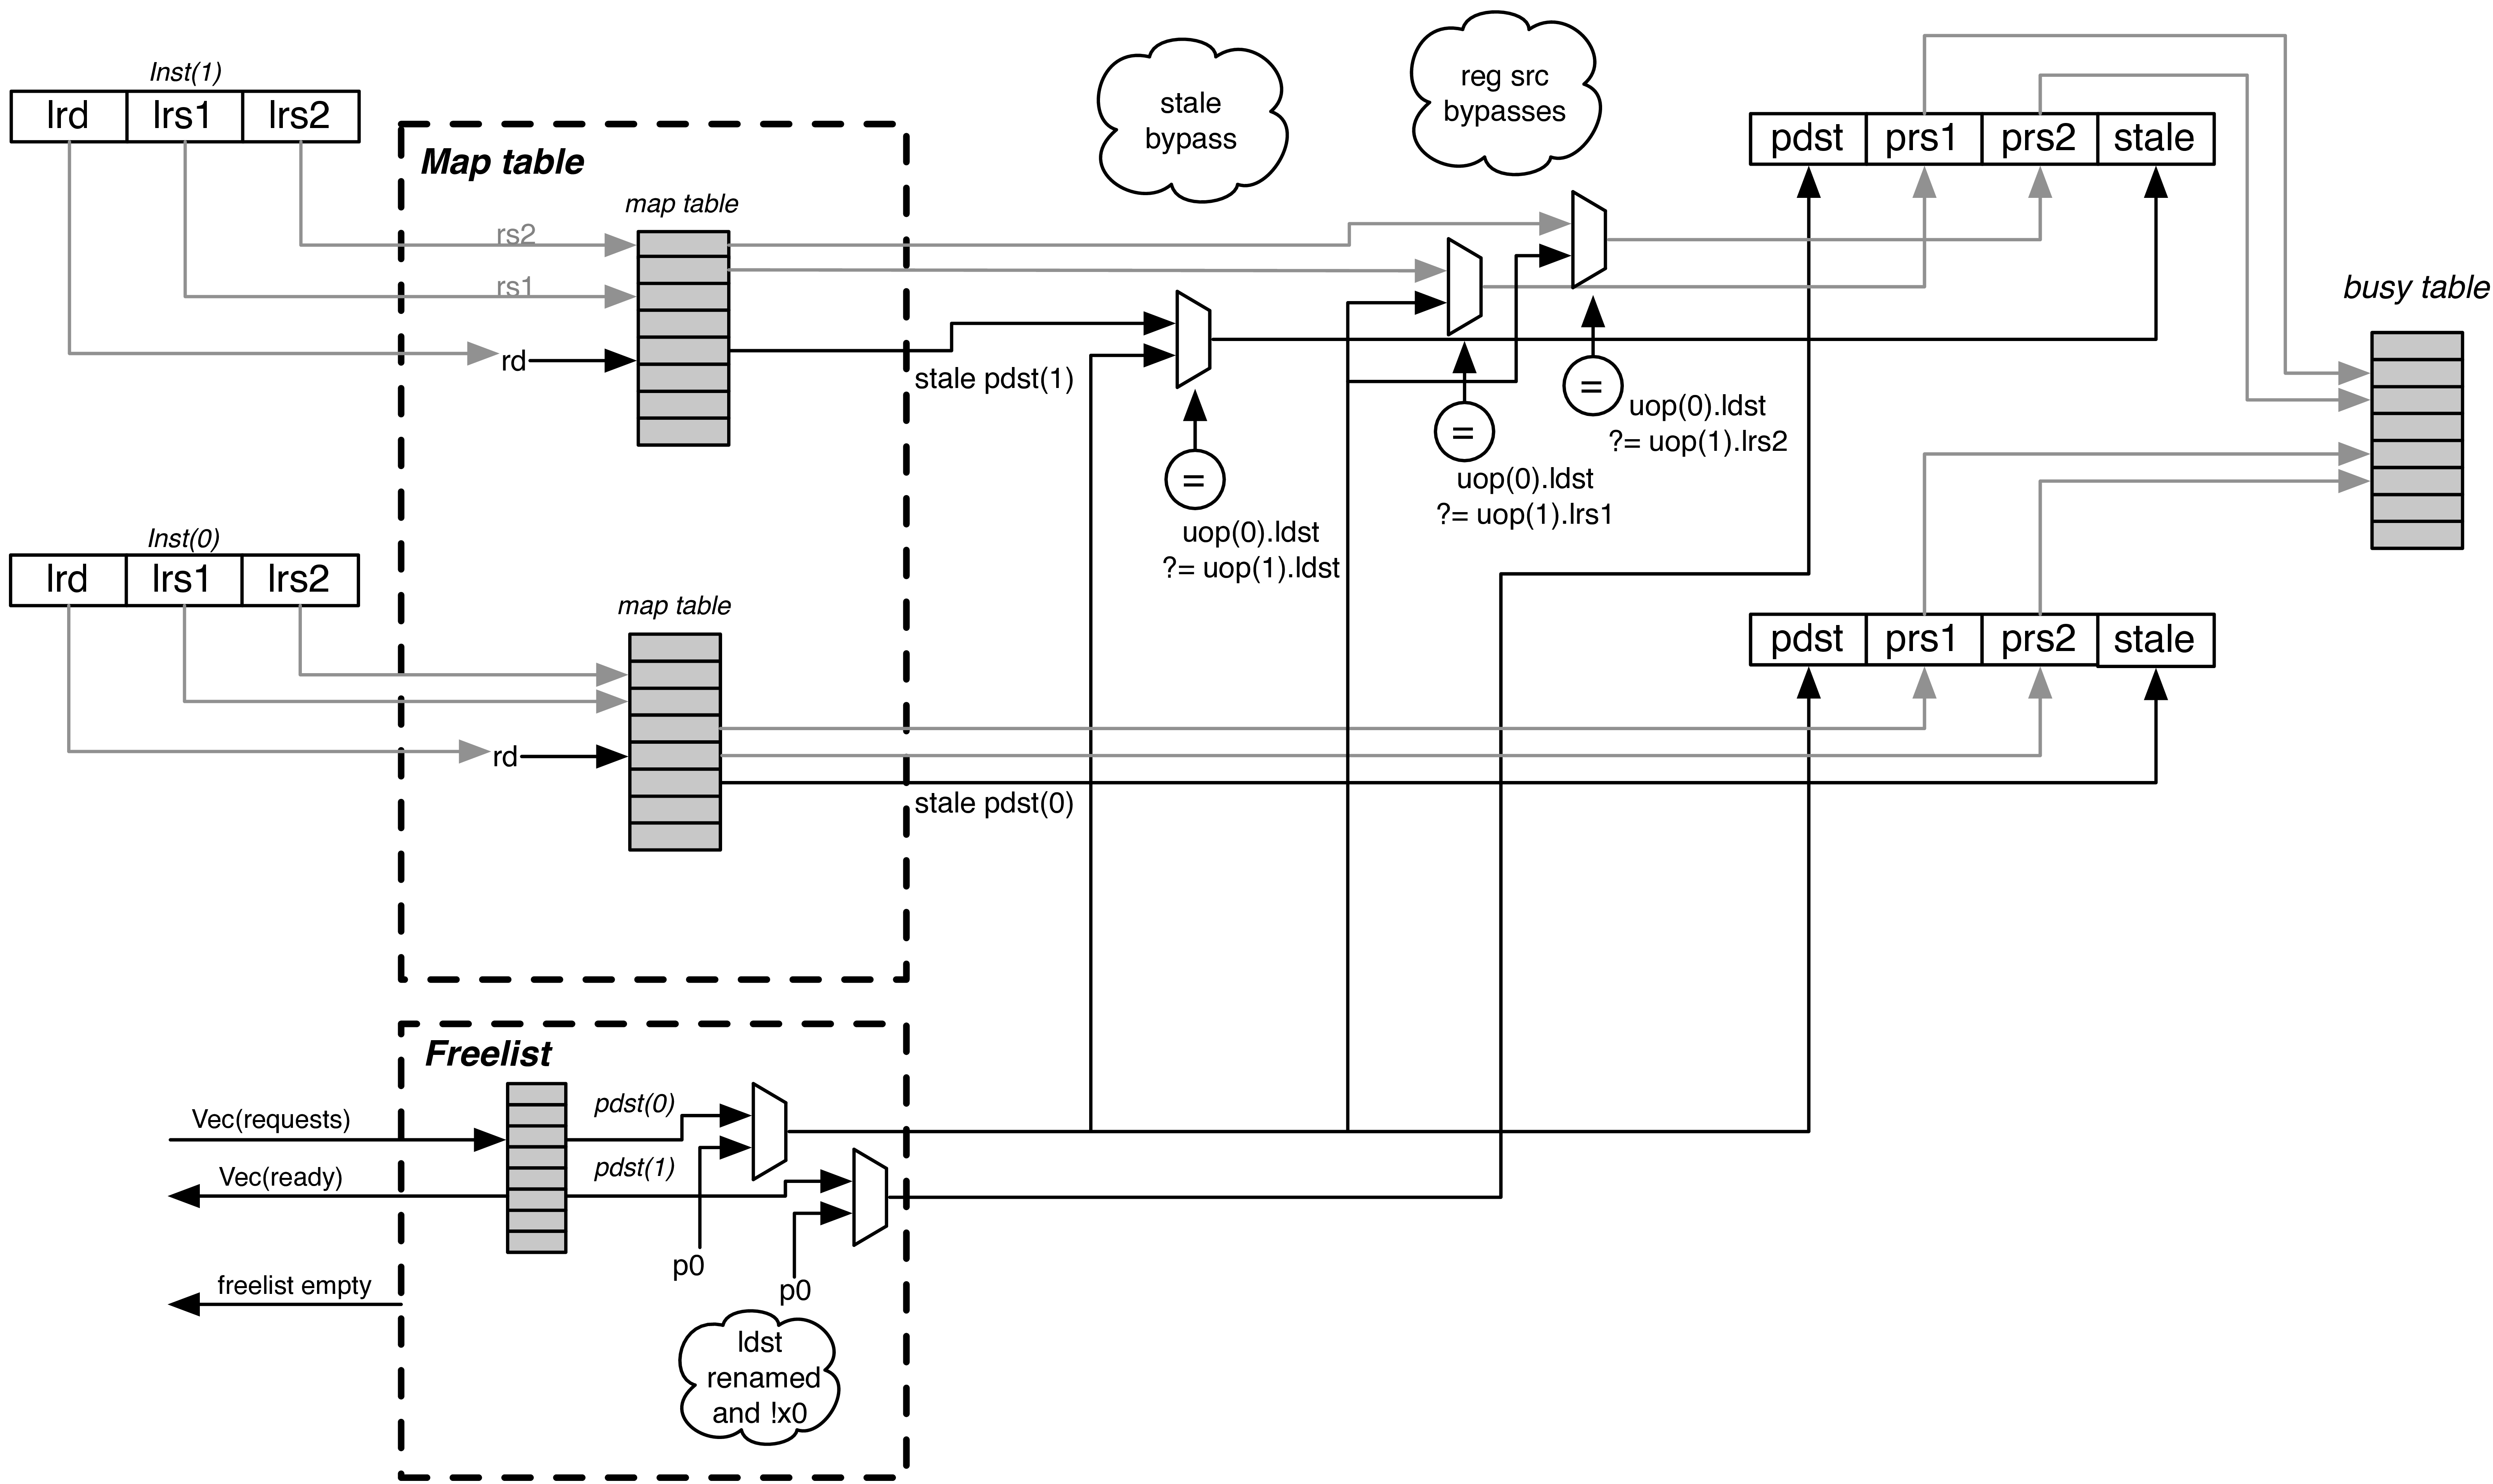
\includegraphics[width=0.8\textwidth]{figure/rename-pipeline.png}
    \caption{Register rename logic\cite{Boom}.}
    \label{fig:rename}
\end{figure}

We use a free list to record the usage of physical registers. When a physical register is assigned to an architecture register, it will be marked as ``busy'' in the free list. On the other hand, when it is retired by the retired instructions, it will be marked as ``free''. Fig.~\ref{fig:mapping} shows the relation between mapping table, free list and rRAT.

\begin{figure}[!htp]
    \centering
    
\includegraphics[width=0.65\textwidth]{figure/map_rename.png}
    \caption{Rename stage with free list, mapping table and rRAT.}
    \label{fig:mapping}
\end{figure}

To avoid data hazards and risks, we use a conservative strategy. When an architectural register $x_a$ is re-assigned to a new physical register $r_b$, its previous physical register $r_a$ will be recorded. Cycles later, when the architectural register $x_a$ is retired by its instruction, its previous physical register $r_a$ will be freed or assigned to another architecture register. At that time, the free list or the mapping table is updated by the new mapping relation. Besides, rRAT is also refreshed by the mapping relation between architectural register $x_a$ and its new physical register $r_b$ so that the rename stage can quickly recover from mis-prediction, interrupts or exceptions.

When a mis-prediction happens, the mapping table and the free list will recover their mapping relation and free stages from rRAT. The recover process takes only one clock cycle, which means that our rename stage can quickly response to mis-prediction, interrupts or exceptions. This feature can reduce our instructions per cycle (IPC) in programs with many branch mis-predictions or interrupts.

\subsection{Dispatch} %sl

Dispatch is the last stage in the frontend and also the last in-order stage. In this part, we write the instructions from the previous stage into the re-order buffer (ROB) the backend and then dispatch these instructions to the corresponding issue units according to the \texttt{iq\_code} field in the uops. We support dispatching 4 instruction at one time. To reduce the logic complexity of input selection in the issue stage, we design our dispatch stage based on collapsing logic, shown in Fig.~\ref{fig:dp-1}. The instructions will always be dispatched to the top space in the inputs of backend without any bubbles.

\begin{figure}[!htp]
    \centering
    \begin{subfigure}{0.45\textwidth}
        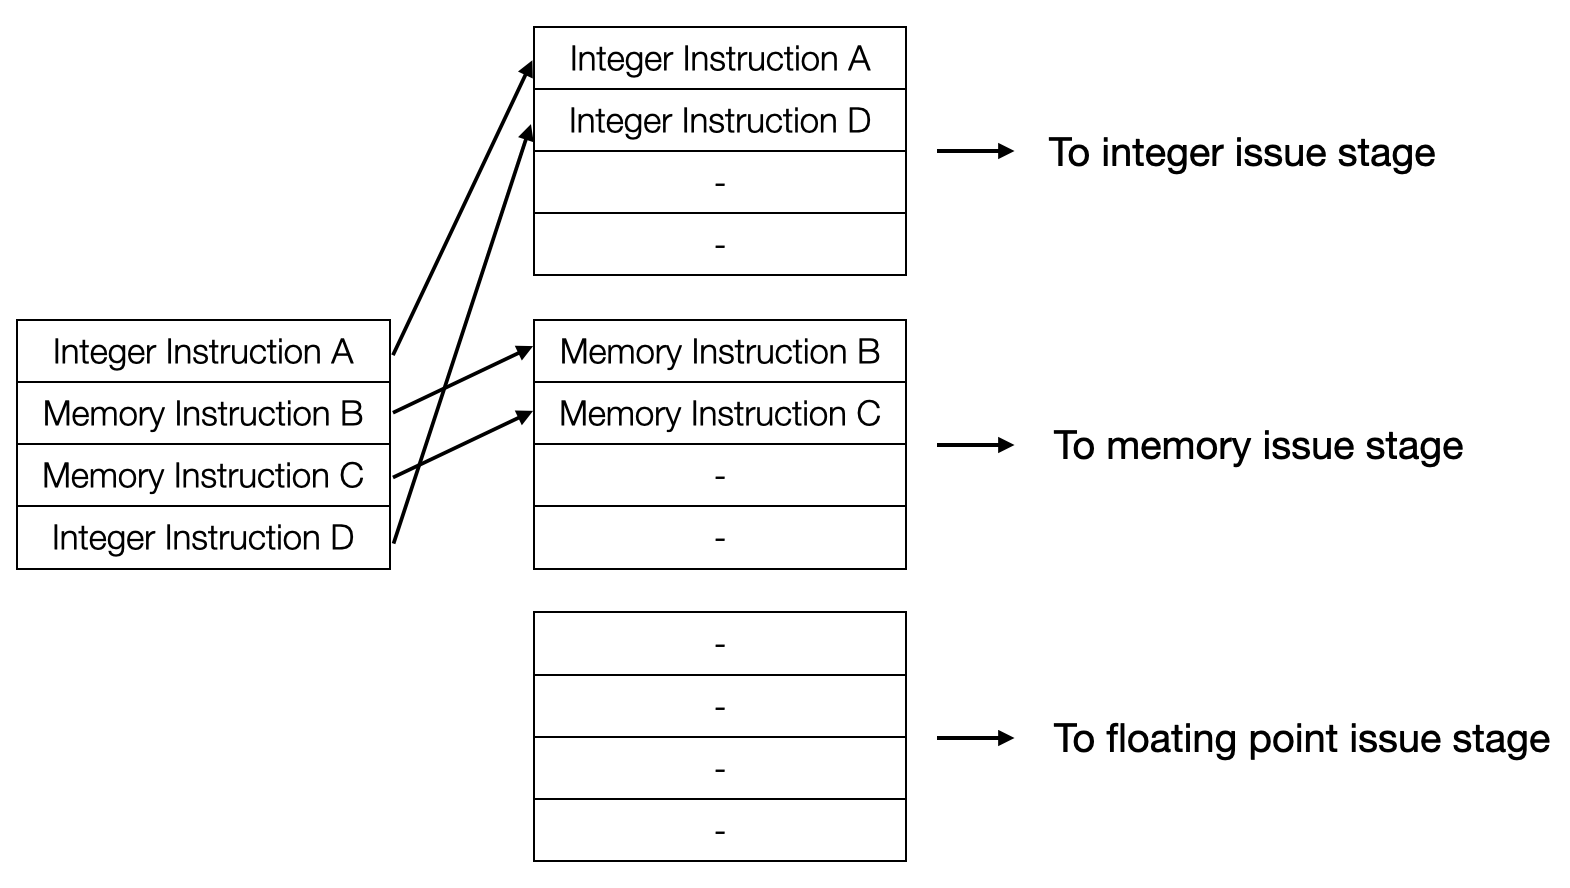
\includegraphics[width=\textwidth]{figure/dispatch.png}
        \caption{Collapsing dispatch logic.}
        \label{fig:dp-1}
    \end{subfigure}
    ~
    \begin{subfigure}{0.45\textwidth}
        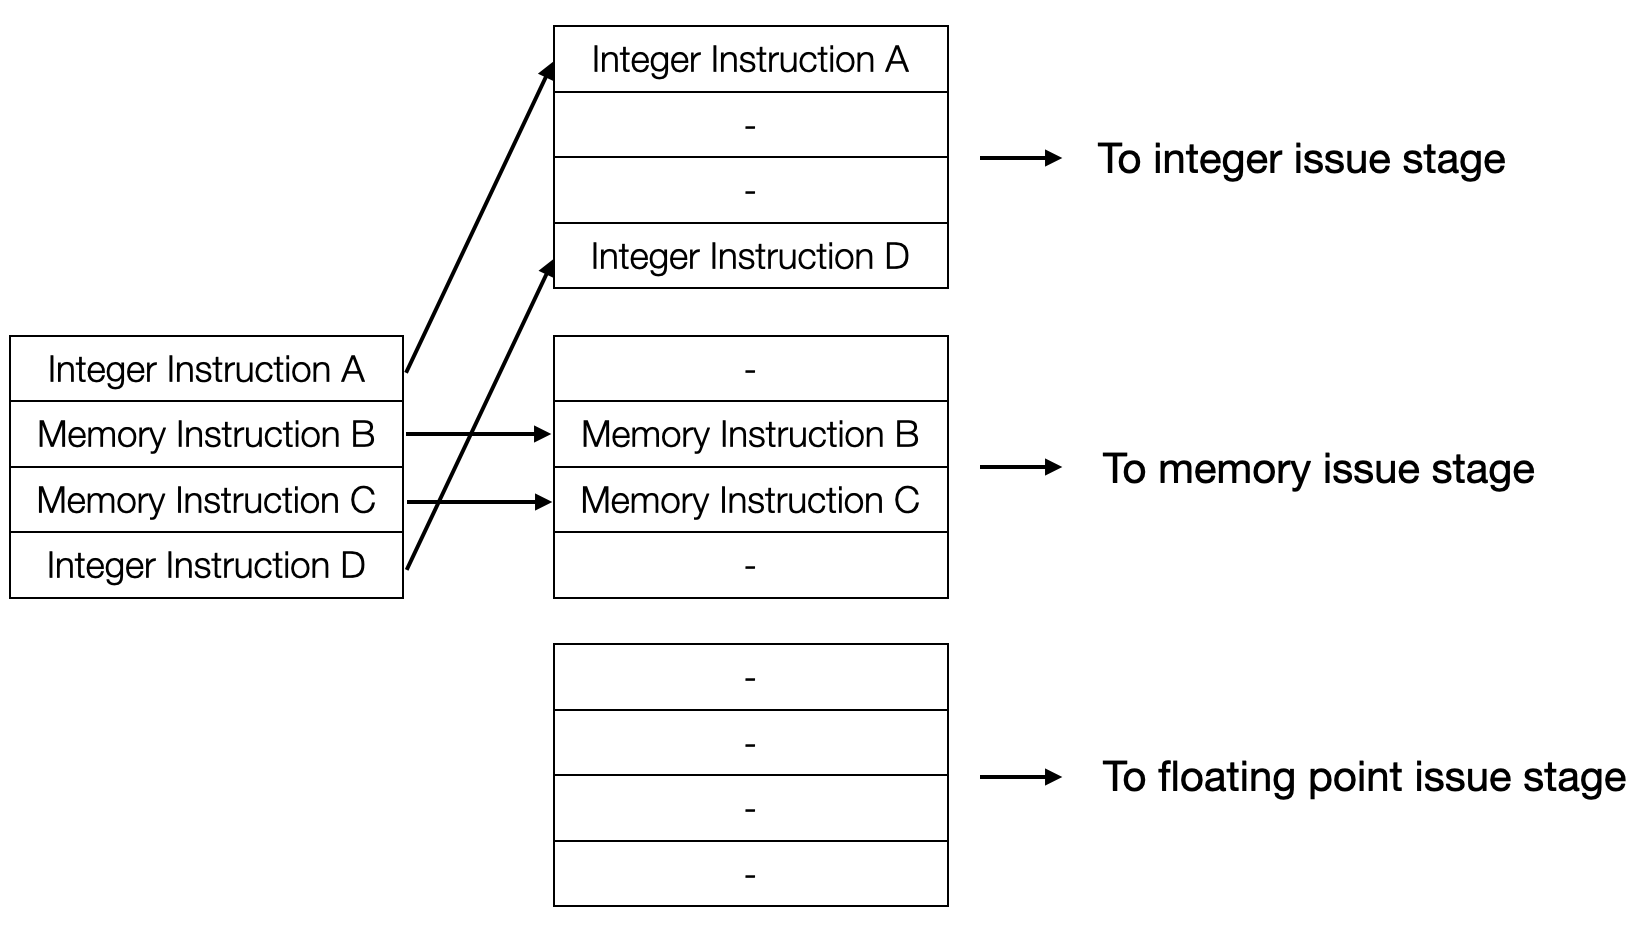
\includegraphics[width=\textwidth]{figure/dispatch-nc.png}
        \caption{Non-collapsing dispatch logic.}
        \label{fig:dp-2}
    \end{subfigure}
    \caption{Two different dispatch logic design.}
    \label{fig:dispatch}
\end{figure}

On the contrary, a non-collapsing dispatcher is shown in Fig.~\ref{fig:dp-2}. The logic is simpler, but it will further complicate the input selection logic and increase the delay in issue stage, especially for memory instructions, which usually require strict memory access order to keep the consistency.


\subsection{Issue} %sl
In this part, we accept the instructions from the frontend, track the data and structure dependency between instructions, select part of the ready instructions and issue them to the register file and the execution units. This is also the critical point between in-order and out-of-order stages in our microarchitecture design, and is the key component to implement out-of-order scheduling algorithm.

In our design, we implement 3 issue units: integer issue unit, memory issue unit and floating point issue unit. All 3 issue units are able to accept four instructions at one time, but the outputs differ, dependent on the design of execution units.

\subsubsection{Issue Unit for Integer \& Floating Point} %sl
We design the input selection logic to assign the input instructions to free space in the issue units. The logic of instruction assignment is simple. We just put the instructions in the free space from top to bottom. Meanwhile, we design the output selection logic to issue instructions whose dependency is ready to the subsequent pipeline stages. The output width depends on the execution width. In our design, we can issue at most 3 integer instructions or 2 floating point instructions simultaneously. Among all the ready instructions, we also select from top to bottom. A simple example of issue unit for integer instructions is shown in Fig.~\ref{fig:iq-int}.

\begin{figure}[!htp]
    \centering
    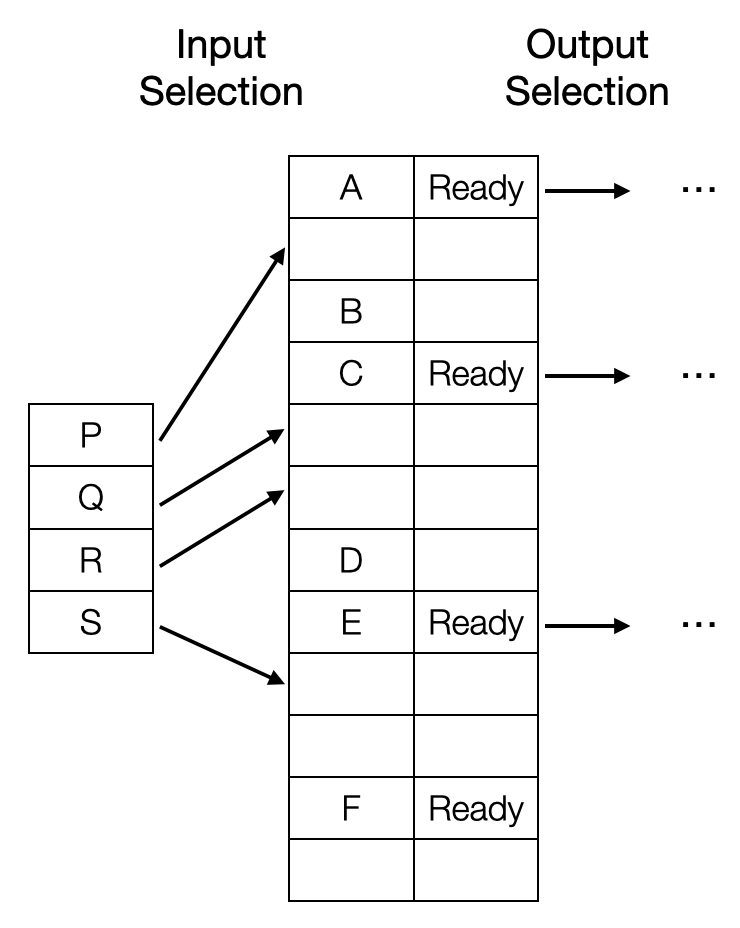
\includegraphics[width=0.3\textwidth]{figure/iq1.png}
    \caption{Example of issue unit logic for integer instructions (L for load and S for store).}
    \label{fig:iq-int}
\end{figure}

\subsubsection{Issue Unit for Memory Access} %sl
Due to the special characteristics of memory access instructions, the selection logic of the issue unit for memory access is different from the logic of the other two issue units. The main principle is to keep the memory consistency, which is a big challenge for out-of-order execution design. It is easy to track data dependency in registers, but it is much more difficult to track the dependency in memory. For example, assuming that the same memory address is stored in the registers \texttt{x1} and \texttt{x2}, for the case that we first store the data to \texttt{[x4]} and then load the data from \texttt{[x3]}, we cannot directly determine whether there exists potential dependency between the two instructions. 

Thus, in our processor design, we use a relatively conservative way to achieve memory consistency. We consider each store instruction as a barrier, i.e., while load instructions can be executed out-of-order, we can issue the store instructions only when it is at the top of our issue unit. As a result, similar to dispatch unit, we design a collapsing structure in the issue unit for memory access. Each time one instruction is issued, all the instructions are ``compressed'' to the top, and the input instructions are added to the tail of the unit. For the output selection logic, if there are remaining store instructions, only the store instruction at the top or the load instructions before any store instructions can be issued.

A simple example is shown in Fig.~\ref{fig:iq-mem}. At the top of the issue unit is a store instruction, which will be issued in this clock cycle. Then all the remaining instructions are pushed to the top, and new instructions are added below.

\begin{figure}[!htp]
    \centering
    \begin{subfigure}{0.4\textwidth}
        \centering
        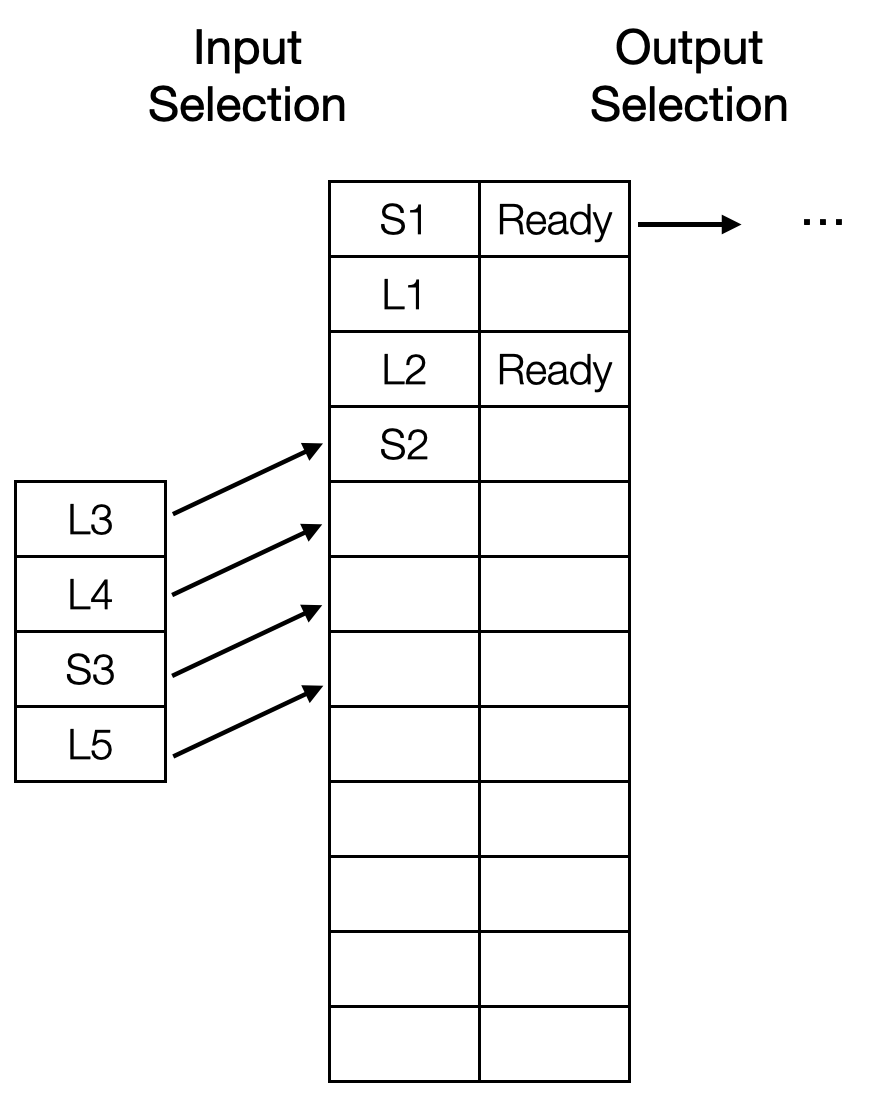
\includegraphics[width=0.75\textwidth]{figure/iq2.png}
        \caption{Example of issue unit logic: stage 1.}
        \label{fig:iq-mem-1}
    \end{subfigure}
    ~
    \begin{subfigure}{0.4\textwidth}
        \centering
        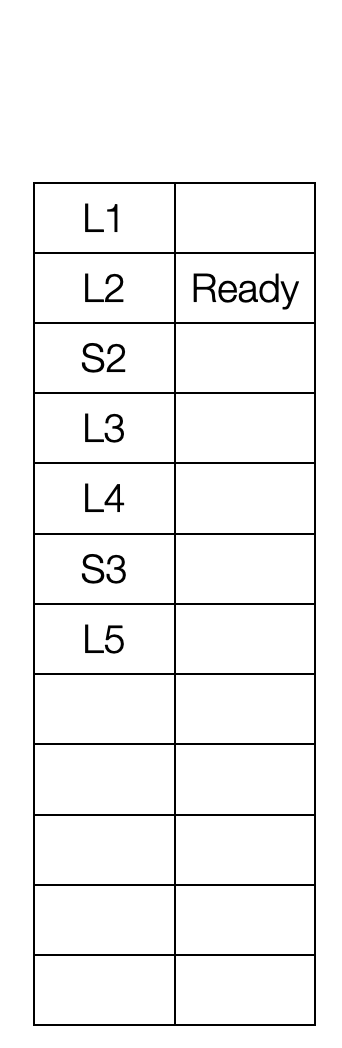
\includegraphics[width=0.3\textwidth]{figure/iq3.png}
        \caption{Example of issue unit logic: stage 2.}
        \label{fig:iq-mem-2}
    \end{subfigure}
    \caption{Example of issue unit logic for memory access.}
    \label{fig:iq-mem}
\end{figure}


\subsubsection{Scoreboard} %sl
Although register renaming may resolve anti-dependency and output dependency, it cannot resolve true dependency, i.e., read-after-write (RAW) dependency, which is usually the crucial bottleneck to further improve instruction level parallelism. In our design, scoreboard is mainly used for tracking data dependency between instructions and sending wake-up signals to the issue units.

The width of scoreboard matches the depth of our physical register file. First, it accepts input from dispatch stage, which is the last in-order stage and sets the busy bits in the scoreboard. Second, it accepts input from write back stage, which clears the busy bits in the scoreboard. Finally, it accepts the query requests from the issue units and returns whether the requiring source registers are ready or not.

Fig.~\ref{fig:sb} shows an example of how scoreboard helps to track RAW dependency between two instructions. Here the second instruction depends on the result of the first instruction. First, when the two instructions enter the dispatch stage, set both \texttt{X} and \texttt{Y} as busy, marking them as in-flight instructions (Fig.~\ref{fig:sb-1}). Second, the first instruction is issued to the later stages of the pipeline (Fig.~\ref{fig:sb-2}). Third, when the first instruction is completed and write back to the register file, set \texttt{X} as not busy (Fig.~\ref{fig:sb-3}). At last, as \texttt{X} is not busy any more, the second instruction checks the scoreboard, finding that it is also ready to issue, and we issue it to the register file and corresponding execution units (Fig.~\ref{fig:sb-4}).

\begin{figure}[!htp]
    \centering
    \begin{subfigure}{0.4\textwidth}
        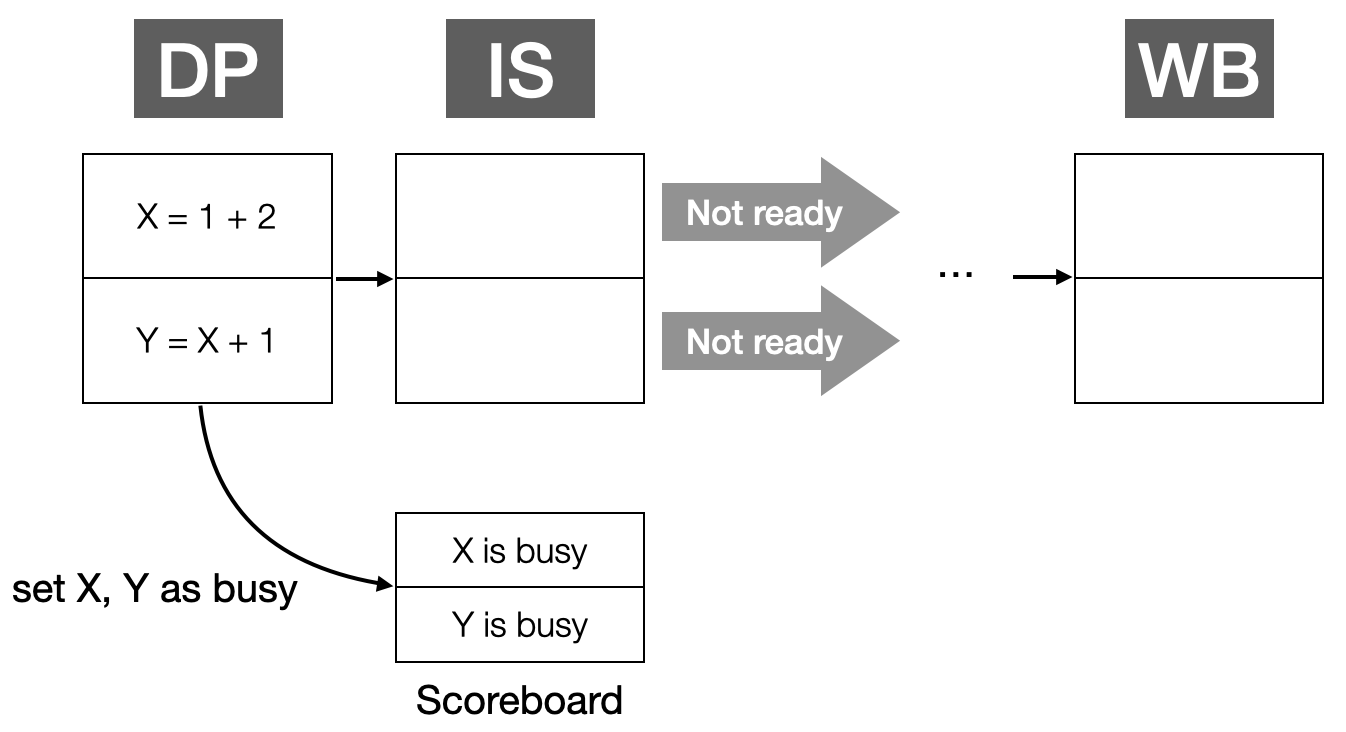
\includegraphics[width=\textwidth]{figure/sb1.png}
        \caption{Example of scoreboard: stage 1.}
        \label{fig:sb-1}
    \end{subfigure}
    ~
    \begin{subfigure}{0.4\textwidth}
        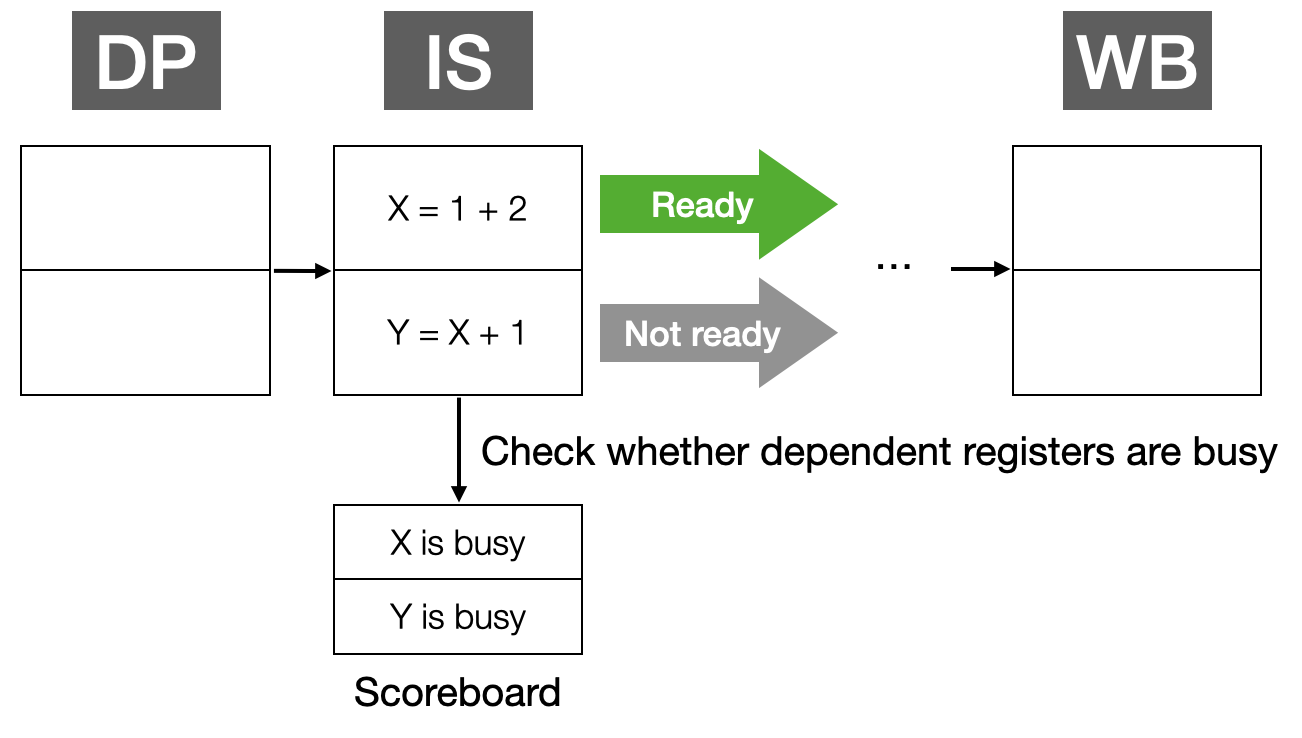
\includegraphics[width=\textwidth]{figure/sb2.png}
        \caption{Example of scoreboard: stage 2.}
        \label{fig:sb-2}
    \end{subfigure}
    
    \begin{subfigure}{0.4\textwidth}
        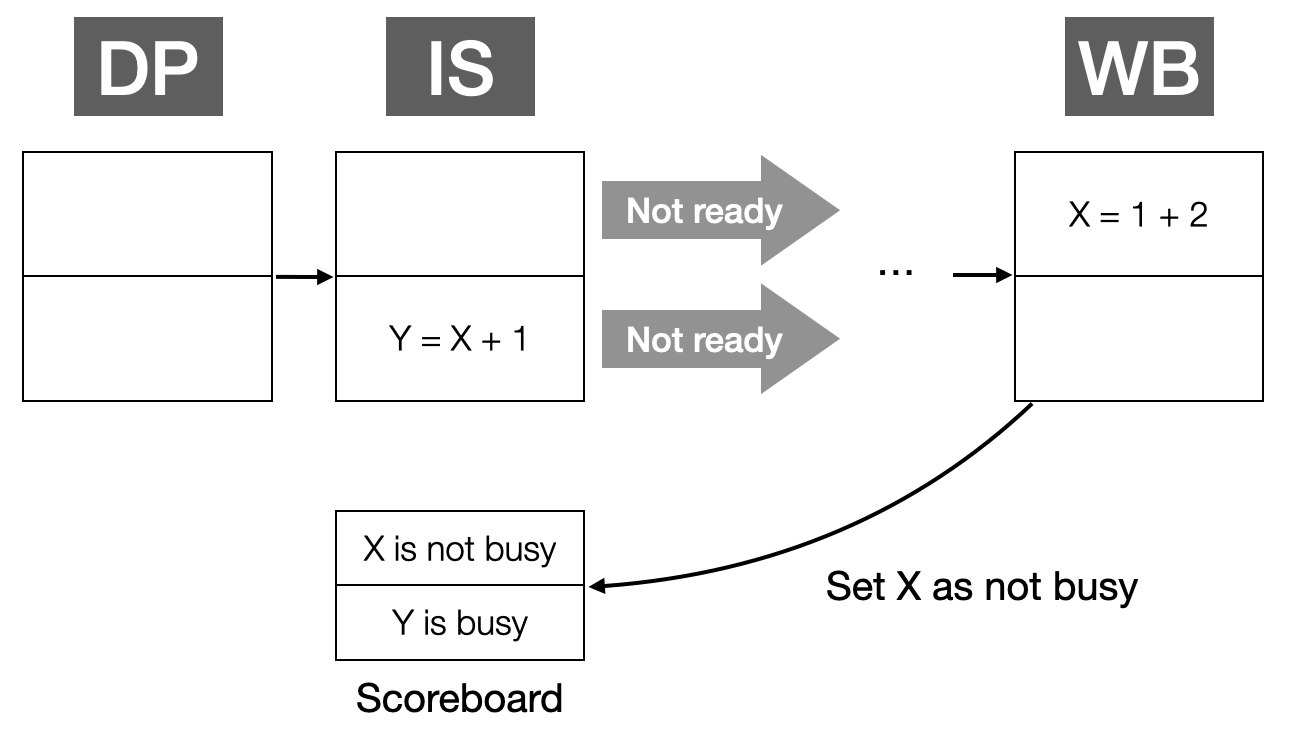
\includegraphics[width=\textwidth]{figure/sb3.png}
        \caption{Example of scoreboard: stage 3.}
        \label{fig:sb-3}
    \end{subfigure}
    ~
    \begin{subfigure}{0.4\textwidth}
        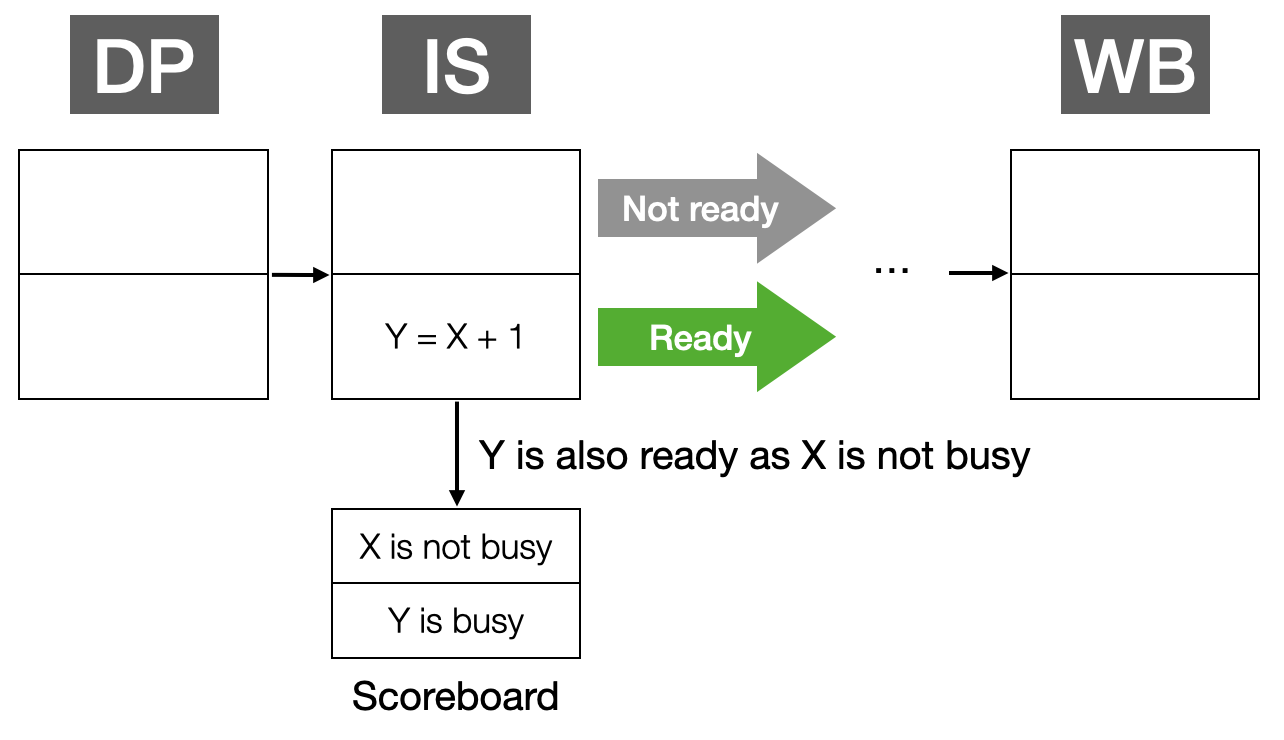
\includegraphics[width=\textwidth]{figure/sb4.png}
        \caption{Example of scoreboard: stage 4.}
        \label{fig:sb-4}
    \end{subfigure}
    \caption{RAW dependency tracking with scoreboard.}
    \label{fig:sb}
\end{figure}

\subsection{Register File} %sl

As mentioned in the register rename part, our processor resolves anti-dependency and output dependency based on physical register file (PRF). In our design, there is only one unified PRF with 128 entries. Bypassing logic is implemented to handle the case that source operands are identical with destination operands. 

Compared to other methods of register renaming, there are several advantages of using PRF. There is no need to move the data frequently, as the data always stays in the PRF. We don't need to add selectors for instructions to determine which register file to use. Furthermore, It is also easy to recover from branch mis-predictions, which helps to further explore the instruction level parallelism and improve the performance.

\subsection{Execution} %sl

An execution pipe is a set of function units. In our microarchitecture design, we have 6 execution pipes in total (3 for integer, 1 for memory access and 2 for floating point), shown in Fig.~\ref{fig:pipe}.

\begin{figure}[!htp]
    \centering
    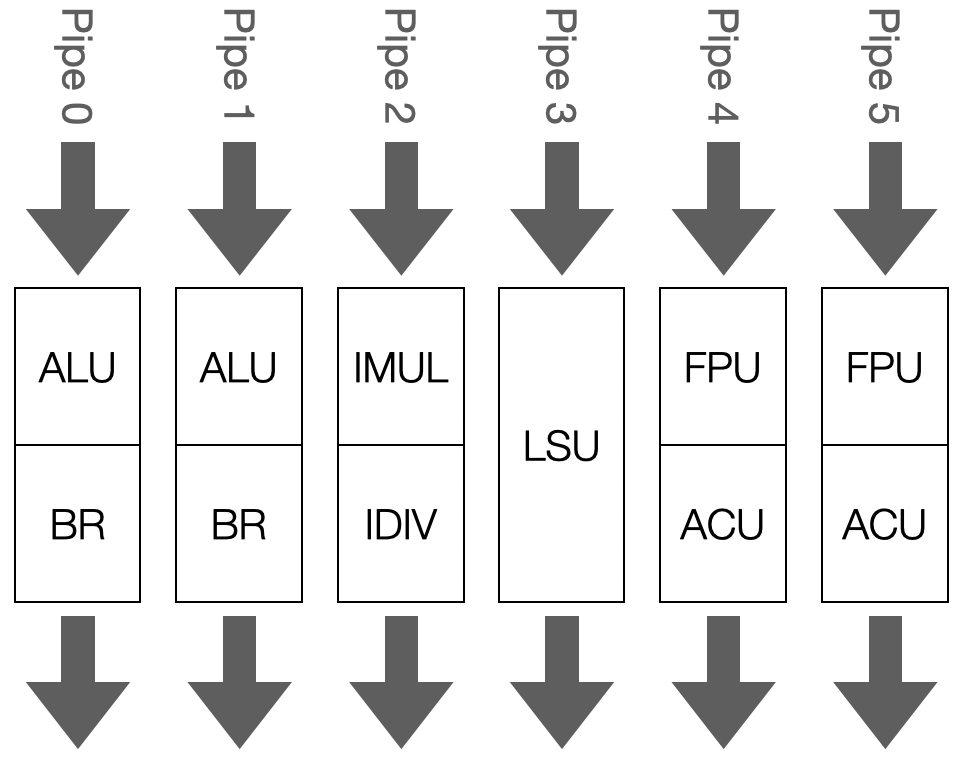
\includegraphics[width=0.4\textwidth]{figure/pipe.png}
    \caption{Execution pipes.}
    \label{fig:pipe}
\end{figure}

\subsubsection{Execution Units for Integer} % sl
There are 3 pipes for integer instructions. Pipe 0 and 1 encapsulate arithmetic logic units (ALU), which perform normal integer arithmetic operations except multiplication and division, and branch units, while pipe 2 is used for integer multiplication and division. ALU and branch units require one clock cycle delay, while integer multiplication and division require more than one clock cycle delay and they are blocking. Instead of using commercial intellectual property (IP) cores, we implement integer multiplier and divider by ourselves based on open source designs.

\subsubsection{Execution Units for Memory Access} %sl
Pipe 3 is for memory access, i.e., load and store instructions, and it is blocking. When a load or store instruction enter this pipe, the processor will send the address, write-enable signal, data to be written and its size (if applicable) to the memory, and receive the data and valid signal from the memory.

\subsubsection{Execution Units for Floating Point} %sj
There are 2 pipes for floating point instructions. Both pipe 4 and 5 encapsulate floating point units (FPU) and approximate computing units (ACU). Each pipe consist of two calculation units, one for general calculation and the other for specialization calculation. The general one can calculate add, sub, sum, sign extension and type transformation. The specialization one can only calculate some special operations. For example, Pipe 4 is specialized for multiplication between floating points, while Pipe 5 is designed for division and square root operation between floating points.

For FPGA board verification, we use IP from Xilinx, Inc to test our design. For software verification, we replace commercial IP with C++ program or open-source FPU model.

\subsection{Write Back} %sl

When the instructions are completed, if the destination operand is valid, the results will be written back to the register file and clear the corresponding busy bits in the scoreboard.

\subsection{Commit} %sj
The commit stage is the last stage in the processor to handle instructions. It consists of a re-order buffer (ROB) that tracks the state of all in-flight instructions in the pipeline. Besides, the ROB also records the order of instructions before they are dispatched into issue queues. The ROB is actually a first-in-first-out queue.

When an instruction is renamed and input to the ROB, it will be marked as ``busy'' in the ROB. On the other time, when it is written back by the write-back stage, it informs the ROB and is marked ``not busy''. Once the ``head'' of the ROB is no longer ``busy'', the instruction is committed, and it’s architectural state now visible. Fig.~\ref{fig:rob} shows the structure of the ROB.

\begin{figure}[!htp]
    \centering
    
\includegraphics[width=0.6\textwidth]{figure/rob.png}
    \caption{Re-order buffer (ROB).}
    \label{fig:rob}
\end{figure}

Since the rename has four ways and the write-back stage has six ways, the ROB can push back four instructions and pop up six instructions at the same time. The final circuit should use some special techniques, called interleaving, to satisfied the requirement.

Mis-predictions, and exceptions are handled when they are at the commit head. When mis-predictions and exceptions happen, their following instructions are illegal and their previous instructions are all committed normally. Therefore, the ROB should be cleared and flushed. At that time, the ROB will send the `recover' signal to all stages in the processor.

